\pgfdeclarelayer{background}
\pgfdeclarelayer{foreground}
\pgfsetlayers{background,main,foreground}

\chapter{General Vector Spaces}
\textbf{Note}: this chapter will be taught only if time permits.

In this chapter we will introduce a more general and abstract approach to vectors and linear transformations. While the approach is more rigorous in its mathematical approach than previous chapters, it is still by no means a formal text on the subject.

\section{$\Rs{n}$ as a Vector Space}
Vectors have the follows properties (some of them may seem quite obvious, but are nontheless important as we will see soon):
\begin{itemize}
  \item The addition of any two vectors is also a vector (closure under addition).
    \begin{example}
      For $\vec{u}=\colvec{3}{3}{-1}{0}, \vec{v}=\colvec{3}{4}{1}{2}$ (both in $\Rs{3}$), the resulting vector $\vec{u}+\vec{v} = \colvec{3}{7}{0}{2}$ is also a vector in $\Rs{3}$.
    \end{example}
  \item For any two vectors $\vec{u},\vec{v}$: $\vec{u}+\vec{v} = \vec{v}+\vec{u}$ (i.e. vector addition is commutative).
    \begin{example}
      For the same vectors as above, $\vec{u}+\vec{v}=\vec{v}+\vec{u}=\colvec{3}{7}{0}{2}$.
    \end{example}
  \item For any three vectors $\vec{u},\vec{v}$ and $\vec{w}$: $\left(\vec{u}+\vec{v}\right)+\vec{w} = \vec{u}+\left( \vec{v}+\vec{w} \right)$ (i.e. vector addition is associative).
    \begin{example}
      The vectors $\vec{u}=\colvec{2}{0}{1},\ \vec{v}=\colvec{2}{3}{7},\ \vec{w}=\colvec{2}{1}{-4}$ can be added as follows:
      \begin{equation*}
        \left[\colvec{2}{0}{1}+\colvec{2}{3}{7}\right]+\colvec{2}{1}{-4} = \colvec{2}{3}{8}+\colvec{2}{1}{-4} = \colvec{2}{4}{4},
      \end{equation*}
      or as follows:
      \begin{equation*}
        \colvec{2}{0}{1} + \left[ \colvec{2}{3}{7} + \colvec{2}{1}{-4} \right] = \colvec{2}{0}{1} + \colvec{2}{4}{3} = \colvec{2}{4}{4},
      \end{equation*}
      which yields the same result.
    \end{example}
  \item The zero vector $\vec{0}$ has the property that for any vector $\vec{v}$, $\vec{v}+\vec{0} = \vec{0}+\vec{v} = \vec{v}$.
    \begin{example}
      \begin{equation*}
        \colvec{3}{7}{1}{0} + \colvec{3}{0}{0}{0} = \colvec{3}{0}{0}{0} + \colvec{3}{7}{1}{0} = \colvec{3}{7}{1}{0}.    
      \end{equation*}
    \end{example}
  \item For any vector $\vec{u}$ there exist a vector $\vec{v}$ such that $\vec{u}+\vec{v} = \vec{v}+\vec{u} = \vec{0}$. Specifically, this is the vector $\vec{v}=-\vec{u}$.
    \begin{example}
      \begin{equation*}
        \colvec{3}{7}{1}{0} + \colvec{3}{-7}{-1}{0} = \colvec{3}{-7}{-1}{0} + \colvec{3}{7}{1}{0} = \colvec{3}{0}{0}{0}.
      \end{equation*}
    \end{example}
\end{itemize}

In addition, the follows properties also exist together with scalars:
\begin{itemize}
  \item For any vector $\vec{v}$ and any scalar $\alpha$, the product $\alpha\cdot\vec{v}$ is also a vector (closure under multiplication).
    \begin{example}
      The $\Rs{4}$ vector $\vec{v}=\colvec{4}{1}{-3}{2}{7}$ and the scalar $\alpha=-2$ multiplied together give
      \begin{equation*}
        \alpha\vec{v} = -2\colvec{4}{1}{-3}{2}{7} = \colvec{4}{-2}{6}{-4}{-14},
      \end{equation*}
      which is also a vector in $\Rs{4}$.
    \end{example}
  \item For any two vectors $\vec{u}, \vec{v}$ and any scalar $\alpha$: $\alpha\cdot\left( \vec{u}+\vec{v} \right) = \alpha\cdot\vec{u} + \alpha\cdot\vec{v}$.
  \item For any vector $\vec{v}$ and any scalars $\alpha, \beta$: $\left( \alpha+\beta \right)\cdot\vec{v} = \alpha\cdot\vec{v} + \beta\cdot\vec{v}$.
  \item For any vector $\vec{v}$ and sny scalars $\alpha, \beta$: $\alpha\cdot\left( \beta\cdot\vec{v} \right) = \left( \alpha\cdot\beta \right)\cdot\vec{v}$.
  \item For any vector $\vec{v}$: $1\cdot\vec{v} = \vec{v}$.
\end{itemize}

Any set of elements obeying these properties, using any kind of operation between two of its elements (here the vector addition operation) and another operation between one element and a scalar (here scalar-vector multiplication) is called a \emph{vector space}\index{Vector space}. The scalars must be of an algebraic structure called a \emph{field}\index{Field}, which we will not define here and assume for simplicity that is either $\mathbb{R}$ or $\mathbb{C}$.

\section{Examples of Vector Spaces}
\subsection{Polynomials of Degree $\mathbf{\leq n}$}
A polynomial of a degree $n$ is an expression of the form
\begin{align*}
  P(x) &= a_{0} + a_{1}x + a_{2}x^{2} + \dots + a_{n}x^{n}\\
  &= \sum\limits_{k=0}^{n} a_{k}x^{k},
\end{align*}
where $a_{0}, a_{1}, \dots, a_{n}$ are called the \emph{polynomial coefficients}\index{Polynomial coefficients}.

When the value of a polynomial coefficient $a_{i}$ is zero, we don't write the corresponding component.
\begin{example}
  The 3rd degree polynomial with coefficients
  \begin{equation*}
    a_{0}=2,\ a_{1}=-5,\ a_{2}=0,\ a_{3}=1
  \end{equation*}
  is written explicitly as
  \begin{equation*}
    p(x) = x^{3}-5x+2.
  \end{equation*}
  (notice the descenting power order used here, contrary to the ascending power order used in the definition)
\end{example}

Adding two polynimials together results in another polynomial, since the coefficients are added power-wise:
\begin{align*}
  P(x) &= a_{0} + a_{1}x + a_{2}x^{2} + \dots + a_{n}x^{n},\\
  Q(x) &= b_{0} + b_{1}x + b_{2}x^{2} + \dots + b_{n}x^{n},\\
  \Rightarrow (P+Q)(x) &= (a_{0}+b_{0}) + (a_{1}+b_{1})x + (a_{2}+b_{2})x^{2} + \dots + (a_{n}+b_{n})x^{n}.
\end{align*}

Multiplying a polynomial by a constant also results in a polynomial, where each of the powers are multiplied by the constant:
\begin{equation*}
  \alpha\cdot P(x) = \alpha a_{0} + \alpha a_{1}x + \alpha a_{2}x^{2} + \dots + \alpha a_{n}x^{n}.
\end{equation*}

\begin{example}
  Adding two polynomials:
  \begin{align*}
    P(x) &= 3x^{2} + 2x - 5,\\
    Q(x) &= 4x^{2} + 7,\\
    \Rightarrow(P+Q)(x) &= (3+4)x^{2} + (2+0)x + (-5+7) = 7x^{2} + 2x + 2.
  \end{align*}

  Multiplying a polynomial by a constant:
  \begin{equation*}
    5\cdot\left( x^{3}-5x^{2}-x+2 \right) = 5x^{3} - 25x^{2} - 5x + 10.
  \end{equation*}
\end{example}

We can use vector notation to represent a polynomial: that way, the $i$-th element of the vector corresponds to the coefficient $a_{i}$.
\begin{example}
  Some polynomials represented as column vectors:
  \begin{align*}
    2x^{5} - 7x^{4} + 3x^{2} - 1 &\Rightarrow \colvec{6}{-1}{0}{3}{0}{-7}{2}\\
    x^{2} - 2x + 1 &\Rightarrow \colvec{3}{1}{-2}{1}\\
    -2x^{7}+5 &\Rightarrow \colvec{8}{5}{0}{0}{0}{0}{0}{0}{-2}
  \end{align*}
\end{example}

It should be fairly obvious by now that polynomials of a degree $\leq n$ (with the addition and scalar multiplication shown here) constitute a vector space.
\begin{challange}
  Prove that the polynomials of a degree $\leq n$ together with the shown addition and scalar multiplication are indeed a vector space.
\end{challange}

\begin{warning}
  It is important to note that polynomials constitute a vector space only when we consider \textbf{all} the polynomials of a degree $\leq n$ in such a way that any polynomial of a lesser degree is considered to have the relevant higher order coefficients equaling zero. Otherwise, we lose the closure in regards to both polynomial addition and multiplication by a scalar.
\end{warning}

The zero-element of the polynomial space is of course the zero-polynomial: $P(x)=0 (a_{0}=a_{1}=a_{2}=\dots=a_{n}=0)$. The inverse of any polynomial can be found by inverting each of its coefficients.

Since the polynomials are a well defined vector space, we can define an inner (dot) product for two polynomials $P(x)=\sum\limits_{k=0}^{n}a_{k}x^{k},\ Q(x)=\sum\limits_{k=0}^{n}b_{k}x^{k}$:
\begin{equation*}
  \langle P, Q \rangle = a_{0}b_{0} + a_{1}b_{1} + a_{2}b_{2} + \dots a_{n}b_{n} = \sum\limits_{k=0}^{n}\left(a_{i}+b_{i}\right)x^{k}.
\end{equation*}
Defining an inner product immidetly gives rise to a concept of orthogonality: if the inner product $\langle P, Q\rangle$ of two \textbf{non-zero} polynimials $P,Q$ is zero, then they are orthogonal. This is usefull in many practical applications.
\begin{example}
  All the polynomials $P^{0}(x) = 1, P^{1}(x)=x, P^{2}(x)=x^{2}, dots, P^{n}(x)=x^{n}$ are orthogonal, similar to how in the space $\Rs{n}$ the standard basis vectors are orthogonal to each other.
  In fact, exactly as with $\Rs{n}$, thes polynomials constitute an orthonormal basis of all polynomials with degree $\leq n$.
\end{example}

Since we can represent polynomials as column vectors, we can also use matrices to transform them. One such matrix is the follows:
\begin{equation*}
  D=\begin{pmatrix}
      0 & 1 & 0 & 0 & \dots & 0\\
      0 & 0 & 2 & 0 & \dots & 0\\
      0 & 0 & 0 & 3 & \dots & 0\\
      \multicolumn{6}{c}{\vdots}\\
      0 & 0 & 0 & 0 & \dots & n\\
      0 & 0 & 0 & 0 & \dots & 0\\
    \end{pmatrix},
\end{equation*}
which represents non other than the differential (derivative) operator!

\begin{example}
  Let's see the results of applying $D$ to the polynimial $P(x)=2x^{3}+5x^{2}-2x+1$:
  \begin{align*}
    D\left[ P \right] &= \begin{pmatrix}
                           0 & 1 & 0 & 0\\
                           0 & 0 & 2 & 0\\
                           0 & 0 & 0 & 3\\
                           0 & 0 & 0 & 0
                         \end{pmatrix}\colvec{4}{1}{-2}{5}{2}\\
                         &= \colvec{4}{\cancel{0\cdot1} + 1\cdot(-2) + \cancel{0\cdot5} + \cancel{0\cdot2}}{\cancel{0\cdot1} + \cancel{0\cdot(-2)} + 2\cdot5 + \cancel{0\cdot2}}{\cancel{0\cdot1} + \cancel{0\cdot(-2)} + \cancel{0\cdot5} + 3\cdot2}{\cancel{0\cdot1} + \cancel{0\cdot(-2)} + \cancel{0\cdot5} + \cancel{0\cdot2}}\\
                         &= \colvec{4}{-2}{10}{6}{0}
  \end{align*}
  The resulting represents the polynomial $Q(x)=6x^{2} + 10x -2$, which is indeed the derivative of $P(x)$ (with respect to $x$).
\end{example}

Since the derivative operator can be represented by a matrix, it is a \emph{linear operator}\index{Linear operator} (at least for polynomials of degree $\leq n$).

\begin{challange}
  Show that the derivative operator is a linear operator for any single variable real function.
\end{challange}

\subsection{Real Valued Functions}
The set of real functions in the interval $\left[ a,b \right]$ (where $a,b\in\mathbb{R}$, but could also be $-\infty$ and $\infty$, respectively) is a vector space together with function addition and multiplication by a real number:
\begin{itemize}
  \item For any real functions $f, g$ in $\left[ a,b \right]$, the sum $f+g$ is also a function.
        \begin{example}
          The functions $f(x)=x^{2}-2e^{x}, g(x)=\sin(3x)-4x^{2}$ can be added together to yield
          \begin{equation*}
            \left( f+g \right)(x) = -3x^{2}-2e^{x}+\sin(3x),
          \end{equation*}
          which is also a real function in $\left[ a,b \right]$.
        \end{example}
  \item Multiplying a real function $f$ by a real scalar $\alpha$ also yields a real function.
        \begin{example}
          Multiplying the real function $f(x)=5\log(x)-\frac{2}{x^{3}}$ by $\alpha=7$ yields
          \begin{equation*}
            \left( \alpha f \right)(x) = 35\log(x)-\frac{14}{x^{3}},
          \end{equation*}
          which is also a real function in $\left[ a,b \right]$.
        \end{example}
\end{itemize}

The rest of the criteria for a vector space are also fulfilled.
\begin{challange}
  Show that the rest of the criteria are indeed fulfilled.
\end{challange}

The dimensionality of this space is infinite. This can be shown by considering the interval $\left[ a,b \right]$ to be discrete with $n$ values, i.e.
\begin{equation*}
  \left\{ x_{1}, x_{2}, \dots, x_{n} \right\},
\end{equation*}
where $x_{1}=a, x_{n}=b$. Then, when discussing functions, we look at their values only in these discrete points:
\begin{figure}[H]
  \centering
  \begin{tikzpicture}[declare function={fun(\x) = (0.3*\x)^3-(0.25*\x)^2-0.2*\x+3;}]
    \foreach [count=\xi] \x in {-4,...,4}{
      \begin{pgfonlayer}{background}
        \draw[-, dashed, black!30] (\x,0) to (\x,4);
        \node at (\x+0.05, -0.5) {$x_{\xi}$};
        \draw[-, very thick] (\x,0) to (\x,-0.15);
      \end{pgfonlayer}
      \begin{pgfonlayer}{foreground}
        \node[fill=white, draw=col1, thick, rounded corners] (f\xi) at (\x,{fun(\x)+(-1)^(\xi+1)*1.2}) {$f(x_{\xi})$};
        \filldraw[fill=col3!50, draw=black, thick] (\x, {fun(\x)}) circle (0.05);
        \draw[->, thick] (f\xi) -- (\x, {fun(\x)+(-1)^(\xi+1)*0.15});
      \end{pgfonlayer}
    }
    \begin{pgfonlayer}{main}
      \draw[<->, very thick] (-5,0) to (5,0) node [right] {$x$};
      \draw[domain=-4:4, samples=50, col1, very thick] plot (\x, {fun(\x)});
    \end{pgfonlayer}
  \end{tikzpicture}
\end{figure}

In this context, a function can be written as a vector with each component $f_{i}$ having the value of the function in the respective $x_{i}$:
\begin{equation*}
  \bm{f}=\colvec{4}{f(x_{1})}{f(x_{2})}{\vdots}{f(x_{n})}.
\end{equation*}

This sets implicitly a basis
\begin{equation*}
  B=\left\{ \colvec{4}{1}{0}{\vdots}{0}, \colvec{4}{0}{1}{\vdots}{0}, \dots, \colvec{4}{0}{0}{\vdots}{1} \right\}.
\end{equation*}

Now we can increase the number of points $n$, and at infinity we will get the complete function:

\begin{figure}[H]
  \centering
  \begin{tikzpicture}[declare function={fun(\x) = (0.3*\x)^3-(0.25*\x)^2-0.2*\x+3;}]
    \foreach [count=\xi] \x in {-4,...,4}{
      \begin{pgfonlayer}{background}
        \draw[-, dashed, black!10] (\x,0) to (\x,4);
        \draw[-, very thick] (\x,0) to (\x,-0.15);
      \end{pgfonlayer}
      \begin{pgfonlayer}{foreground}
        \filldraw[fill=col3!50, draw=black, thick] (\x, {fun(\x)}) circle (0.05);
      \end{pgfonlayer}
    }
    \begin{pgfonlayer}{main}
      \draw[<->, very thick] (-5,0) to (5,0) node [right] {$x$};
      \draw[domain=-4:4, samples=50, col1, very thick] plot (\x, {fun(\x)});
    \end{pgfonlayer}
    \node at (-3.5,3.5) {$n=\xi$};
  \end{tikzpicture}

  \vspace{5mm}
  \begin{tikzpicture}[declare function={fun(\x) = (0.3*\x)^3-(0.25*\x)^2-0.2*\x+3;}]
    \foreach [count=\xi] \x in {-4,-3.5,...,4}{
      \begin{pgfonlayer}{background}
        \draw[-, dashed, black!10] (\x,0) to (\x,4);
        \draw[-, very thick] (\x,0) to (\x,-0.15);
      \end{pgfonlayer}
      \begin{pgfonlayer}{foreground}
        \filldraw[fill=col3!50, draw=black, thick] (\x, {fun(\x)}) circle (0.05);
      \end{pgfonlayer}
    }
    \begin{pgfonlayer}{main}
      \draw[<->, very thick] (-5,0) to (5,0) node [right] {$x$};
      \draw[domain=-4:4, samples=50, col1, very thick] plot (\x, {fun(\x)});
    \end{pgfonlayer}
    \node at (-3.5,3.5) {$n=\xi$};
  \end{tikzpicture}

  \vspace{5mm}
  \begin{tikzpicture}[declare function={fun(\x) = (0.3*\x)^3-(0.25*\x)^2-0.2*\x+3;}]
    \foreach [count=\xi] \x in {-4,-3.75,...,4}{
      \begin{pgfonlayer}{background}
        \draw[-, dashed, black!10] (\x,0) to (\x,4);
        \draw[-, very thick] (\x,0) to (\x,-0.15);
      \end{pgfonlayer}
      \begin{pgfonlayer}{foreground}
        \filldraw[fill=col3!50, draw=black, thick] (\x, {fun(\x)}) circle (0.05);
      \end{pgfonlayer}
    }
    \begin{pgfonlayer}{main}
      \draw[<->, very thick] (-5,0) to (5,0) node [right] {$x$};
      \draw[domain=-4:4, samples=50, col1, very thick] plot (\x, {fun(\x)});
    \end{pgfonlayer}
    \node at (-3.5,3.5) {$n=\xi$};
  \end{tikzpicture}

  \vspace{5mm}
  \begin{tikzpicture}[declare function={fun(\x) = (0.3*\x)^3-(0.25*\x)^2-0.2*\x+3;}]
    \foreach [count=\xi] \x in {-4,-3.9,...,4}{
      \begin{pgfonlayer}{background}
        \draw[-, dashed, black!10] (\x,0) to (\x,4);
        \draw[-, very thick] (\x,0) to (\x,-0.15);
      \end{pgfonlayer}
      \begin{pgfonlayer}{foreground}
        \filldraw[fill=col3!50, draw=black, thick] (\x, {fun(\x)}) circle (0.05);
      \end{pgfonlayer}
    }
    \begin{pgfonlayer}{main}
      \draw[<->, very thick] (-5,0) to (5,0) node [right] {$x$};
      \draw[domain=-4:4, samples=50, col1, very thick] plot (\x, {fun(\x)});
    \end{pgfonlayer}
    \node at (-3.5,3.5) {$n=\xi$};
  \end{tikzpicture}
\end{figure}

Since each function has an infinite amount of components, the basis is also infinite, and is composed of dirac-detla "functions". The dirac delta is defined as:
\begin{equation*}
  \delta(x) = \begin{cases} +\infty & x=0,\\ 0 & x\neq0 \end{cases},
\end{equation*}
i.e. it is inifite at $x=0$ and zero anywhere else. It can be visualized as so:
\begin{figure}[H]
  \centering
  \begin{tikzpicture}
    \draw[<->, very thick] (-5,0) to (5,0) node [right] {$x$};
    \draw[->, very thick, col1] (0,0) to (0,3);
    \node at (0, -0.5) {$0$};
  \end{tikzpicture}
\end{figure}

This means that the basis is composed of an infinite amount of dirac deltas of the the form
\begin{equation*}
  \delta\left(x-x'\right),
\end{equation*}
where $x'$ is a number in $\left[ a,b \right]$.
\begin{example}
  A graphic representation of $\color{col1}\delta\left( x-3 \right)\color{black}$ and $\color{col2}\delta\left( x+1 \right)\color{black}$:
  \begin{figure}[H]
    \centering
    \begin{tikzpicture}
      \draw[<->, very thick] (-5,0) to (5,0) node [right] {$x$};
      \draw[->, very thick, col1] (3,0) to (3,3) node [left] {$\delta\left( x-3 \right)$};
      \draw[->, very thick, col2] (-1,0) to (-1,3) node [left] {$\delta\left( x+1 \right)$};
      \node at (0, -0.5) {$0$};
      \node at (3, -0.5) {$3$};
      \node at (-1, -0.5) {$-1$};
    \end{tikzpicture}
  \end{figure}
\end{example}

\subsubsection{Spanning the Space}

\subsubsection{Inner Product and Normalization}
We can also define an inner product on this space:
\begin{equation*}
  \dotp{f}{g} = \int\limits_{a}^{b} f(x)g(x)\dif x.
\end{equation*}

This leads to the idea of \emph{orthogonal functions}\index{Orthogonal functions}. 

\begin{example}
  in the interval $\left[ -\pi, \pi \right]$, the functions
  \begin{equation*}
    f(x)=\sin(x),\ g(x)=x^{2}
  \end{equation*}
  have the follows inner product:
  \begin{align*}
    \dotp{f}{g} &= \int\limits_{-\pi}^{\pi}f(x)g(x)\dif x\\
    &=\int\limits_{-\pi}^{\pi}x^{2}\sin(x)\dif x\\
    &= \int\limits_{-\pi}^{0}x^{2}\sin(x)\dif x + \int\limits_{0}^{\pi}x^{2}\sin(x)\dif x\\
    &= \int\limits_{-\pi}^{0}x^{2}\sin(x)\dif x -\int\limits_{-\pi}^{0}x^{2}\sin(x)\dif x\\
    &= 0.
  \end{align*}
  Thus, these two functions are orthogonal in $\left[ -\pi, \pi \right]$.
\end{example}

Recall that in $\Rs{n}$ the norm of a vector is defined as
\begin{equation*}
  \vnorm{v} = \sqrt{\sum\limits_{i=1}^{n}v_{i}^{2}},
\end{equation*}
which can be viewed as
\begin{equation*}
  \vnorm{v} = \sqrt{\sum\limits_{i=1}^{n}\left(v_{i}\cdot v_{i}\right)}.
\end{equation*}
This is exactly the square root of the dot prouct of the vector with itself. Thus, a generalized norm for a vector $\bm{x}$ can be defined using the inner product as follows:
\begin{equation*}
  \left\| \bm{x} \right\| = \sqrt{\dotp{\bm{x}}{\bm{x}}}.
\end{equation*}

Thus, the norm of a real function $f(x)$ over $\left[ a,b \right]$ is:
\begin{align*}
  \left\|f\right\| &= \sqrt{\dotp{f}{f}}\\
  &= \int\limits_{a}^{b}f(x)f(x)\dif x\\
  &= \int\limits_{a}^{b}f^{2}(x)\dif x.
\end{align*}

\begin{example}
  The norm of the Gaussian function $f(x)=e^{-\frac{x^{2}}{2}}$ over $\left( -\infty, \infty \right)$ is
  \begin{align*}
    \left\| f \right\| &= \int\limits_{-\infty}^{\infty}e^{-\frac{x^{2}}{2}}e^{-\frac{x^{2}}{2}}\dif x\\
    &= \int\limits_{-\infty}^{\infty}e^{-\frac{x^{2}}{2}-\frac{x^{2}}{2}}\dif x\\
    &= \int\limits_{-\infty}^{\infty}e^{-x^{2}}\dif x\\
    &= \frac{1}{\sqrt{2\pi}}.
  \end{align*}

  To normalize the function, we divide it by its norm, $\frac{1}{\sqrt{2\pi}}$, which yields the \emph{Normal distribution}\index{Normal distribution}:
  \begin{equation*}
    f(x) = \frac{1}{\sqrt{2\pi}}e^{-\frac{x^{2}}{2}}.
  \end{equation*}
  
  Graphing the normal distribution:
  \begin{figure}[H]
    \centering
    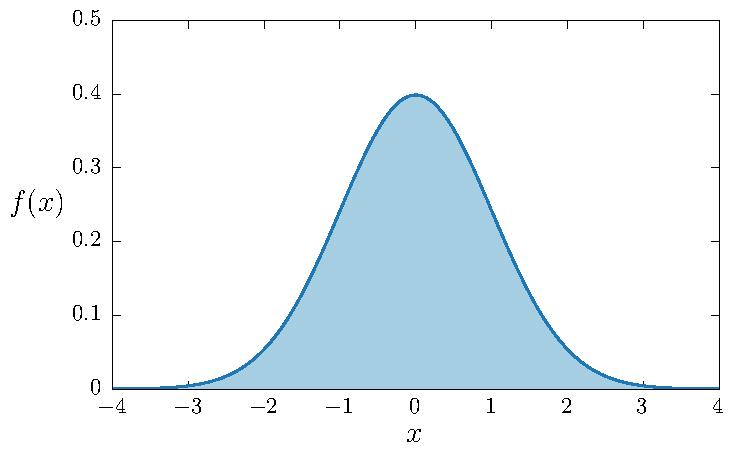
\includegraphics{normal_distribution/normal_distribution.pdf}
  \end{figure}
\end{example}

\subsubsection{Eigenfunctions}
Similar to the eigenvectors of a linear transformation, some linear operators operating on real functions have eigenfunctions: functions that are scaled by a real number when operated on by the operator.
\begin{example}
  The derivative operator $D$ has eigenfunctions. These are of course of the form
  \begin{equation*}
    Df = \lambda f,
  \end{equation*}
  i.e. functions with a derivative that is equal to the function times a scalar. Their form is
  \begin{equation*}
    f(x) = e^{\lambda x},
  \end{equation*}
  as the derivative of an exponential function is
  \begin{equation*}
    \od{f}{x}e^{\lambda x} = \lambda e^{\lambda x} = \lambda f(x).
  \end{equation*}
\end{example}
